\graphicspath{ {./slike/} }
\section{Naloga}\label{sec:jedro}
%
\begin{enumerate}
    \item[i.)] Izmeri in izračunaj resonančno krivuljo za torzijsko nihalo pri dveh različnih dušenjih!
\end{enumerate}

\section{Potrebščine}
\begin{itemize}
    \item Torzijsko nihalo
    \item elektromotor z vzvodom
    \item Štoparica
\end{itemize}

\section{Skica}
Izjemno groba skica ekspirimentalne meritve nihanja. Skica je izjemno slaba ampak ponazarja krog, ki ga odmika polžasta vzmet.

\makebox[0pt][l]{\begin{minipage}{\textwidth}\centering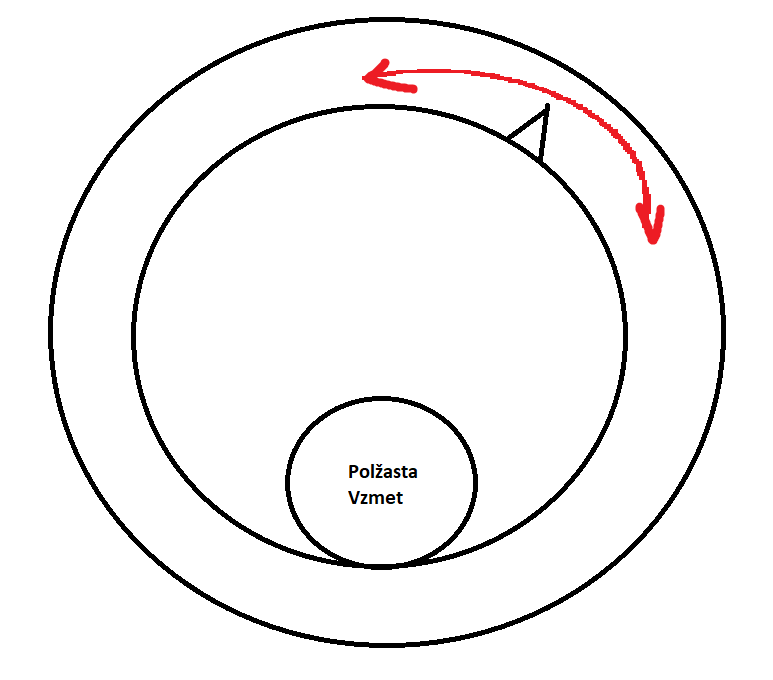
\includegraphics[width=0.8\textwidth]{slike/skica.png}\captionof{figure}{Skica kalorimetra}\end{minipage}}

\section{Meritve}

\begin{itemize}
\centering
\item[]
    \begin{tabular}{|p{1.5cm}|p{1.5cm}|}
        \hline
        \multicolumn{2}{|c|}{Spološnmi podatki}\\
        \hline
        Meritev & Vrednost\\
        \hline
        $T_{sobe}$ & 22,5 C\\
        $RH$ & 57 $\%$ \\
        $P$ & 1016 hPa\\
        \hline
    \end{tabular}
\item[]
    \begin{tabular}{|p{1.5cm}|p{1.5cm}|p{1.5cm}|}
        \hline
        \multicolumn{3}{|c|}{1. Dušeno lastno nihanje meritev 1; n = 5}\\
        \hline
        Meritev & Vrednost L. & Vrednost D.\\
        \hline
        $A_z$ & 97,5 deg & 105 deg\\
        $A_k$ & 75 deg & 82,5 deg\\
        $t$ & 12,7 $s$ & 12,7 $s$\\
        \hline
    \end{tabular}
\item[]
    \begin{tabular}{|p{1.5cm}|p{1.5cm}|p{1.5cm}|}
        \hline
        \multicolumn{3}{|c|}{1. Dušeno lastno nihanje meritev 2; n = 5}\\
        \hline
        Meritev & Vrednost L. & Vrednost D\\
        \hline
        $A_z$ & 30 deg & 37,5 deg\\
        $A_k$ & 15 deg & 22,5deg\\
        $t$ & 12,8 $s$ & 12,8 $s$\\
        \hline
    \end{tabular}
\item[]
    \begin{tabular}{|p{1.5cm}|p{1.5cm}|p{1.5cm}|}
        \hline
        \multicolumn{3}{|c|}{2. Dušeno lastno nihanje meritev 1; n = 4}\\
        \hline
        Meritev & Vrednost L. & Vrednost D.\\
        \hline
        $A_z$ & 82,5 deg & 67,5 deg\\
        $A_k$ & 7.5 deg & 3,8 deg\\
        $t$ & 9,8 $s$ & 10,0 $s$\\
        \hline
    \end{tabular}
\item[]
    \begin{tabular}{|p{1.5cm}|p{1.5cm}|p{1.5cm}|}
        \hline
        \multicolumn{3}{|c|}{2. Dušeno lastno nihanje meritev 2; n = 4}\\
        \hline
        Meritev & Vrednost L. & Vrednost D\\
        \hline
        $A_z$ & 105 deg & 90 deg\\
        $A_k$ & 15 deg & 7.5 deg\\
        $t$ & 10,1 $s$ & 10,2 $s$\\
        \hline
    \end{tabular}
\item[]
    \begin{tabular}{|p{1.5cm}|p{1.5cm}|p{1.5cm}|p{1.5cm}|}
        \hline
        \multicolumn{4}{|c|}{1. Vsiljeno nihanje}\\
        \hline
        Index & Frekvenca [Hz] & Amplituda [deg] & faza\\
        \hline
        1 & 0,10 & 7,5 & 0\\
        2 & 0,20 & 9,8 & 0\\
        3 & 0,30 & 11,3 & $\frac{\pi}{16}$\\
        4 & 0,32 & 12 & $\frac{\pi}{8}$\\
        5 & 0,34 & 13,5 & $\frac{\pi}{4}$\\
        6 & 0,36 & 21 & $\frac{\pi}{2}$\\
        7 & 0,37 & 41,3 & $\frac{\pi}{2}$\\
        \hline
        8 & 0,375 & 180 & $\frac{\pi}{2}$\\
        \hline
        9 & 0,38 & 138,8 & $\frac{\pi}{2}$\\
        10 & 0,40 & 32,3 & $\frac{3\pi}{4}$\\
        11 & 0,42 & 21 & $\pi$\\
        12 & 0,44 & 15 & $\pi$\\
        13 & 0,50 & 7,5 & $\pi$\\
        14 & 0,60 & 3,8 & $\pi$\\
        \hline
    \end{tabular}
\item[]
    \begin{tabular}{|p{1.5cm}|p{1.5cm}|p{1.5cm}|p{1.5cm}|}
        \hline
        \multicolumn{4}{|c|}{2. Vsiljeno nihanje}\\
        \hline
        Index & Frekvenca [Hz] & Amplituda [deg] & faza\\
        \hline
        1 & 0,10 & 6 & 0\\
        2 & 0,20 & 7,5 & 0\\
        3 & 0,30 & 9,8 & 0\\
        4 & 0,32 & 11,3 & $\frac{\pi}{4}$\\
        5 & 0,34 & 13,5 & $\frac{\pi}{4}$\\
        6 & 0,36 & 17,3 & $\frac{\pi}{2}$\\
        7 & 0,38 & 22,5 & $\frac{\pi}{2}$\\
        8 & 0,39 & 30 & $\frac{\pi}{2}$\\
        \hline
        9 & 0,40 & 37,5 & $\frac{\pi}{2}$\\
        \hline
        10 & 0,41 & 22,5 & $\frac{\pi}{2}$\\
        11 & 0,42 & 21 & $\frac{\pi}{2}$\\
        12 & 0,44 & 13,5 & $\frac{3\pi}{4}$\\
        13 & 0,46 & 9,8 & $\frac{3\pi}{4}$\\
        14 & 0,50 & 7,5 & $\pi$\\
        15 & 0,60 & 3,8 & $\pi$\\
        \hline
    \end{tabular}
\item[*]
    faza je fazni zamik
\end{itemize}
\subsection{Metodologija}

Podatke za splošne pogoje smo pridobili s pomočjo stenskega aparata za merjenje rleativne vlažnosti, pritiska in teperature. Pogoji v sobi so ob začetku in kocu bili enaki. S pomočjo posebnega elektromotorja smo na vzmet inducirali sinusno stiskanje in raztezanje vzmeti, odmik smo merili vizualno. Privzeli smo, da je poskus ponovljiv, ter da da vedno iste rezultate, zato smo posebaj merili čas petih nihajev ter amplitudo petega nihaja. Tu se lahko pojavi sistemska napaka. Posebno smo merili vrednosti za desni ekstrem nihala ter levi ekstrem nihala.

\section{Obdelava meritev}
Za izračun lastne dušene frekvence nihala smo uporabili smo uporabili naslednjo enačbo, da smo dobili rezultate:

\subsection{Lastna dušena frekvenca brez dodatnega dušila}

\centering \Large
\begin{equation}
    \omega_d = \frac{2\pi}{t_0}; t_0 = \frac{\overline{t}}{n}
\end{equation}
\raggedright \normalsize
\centering \Large
\begin{equation}
    \omega_d = \frac{2\pi n}{\overline{t}}
\end{equation}
\raggedright \normalsize
\centering \Large
\begin{equation}
    \omega_d = 2,5 * (1\pm 0,004) s^{-1}
\end{equation}
\raggedright \normalsize

\subsection{Lastna dušena frekvenca z dodatnim dušilom}

Uporabimo enačbe iz prejšnjega računa ter dobimo:

\centering \Large
\begin{equation}
    \omega_d = 2,5 * (1\pm 0,02) s^{-1}
\end{equation}
\raggedright \normalsize

\subsection{Koeficient dušena brez dodatnega dušila}

\centering \Large
\begin{equation}
    \beta = \frac{\omega_d}{2\pi n}\ln{\frac{A_0}{A_n}}
\end{equation}
\raggedright \normalsize
\centering \Large
\begin{equation}
    \overline{\beta} = 0,03 * (1\pm0) s^{-1}
\end{equation}
\raggedright \normalsize

Opozorilo: napaka pri $\overline{\beta}$ je reda $10^{-5}$ in ne zares $0$.

\subsection{Koeficient dušena z dodatnim dušilom}

\centering \Large
\begin{equation}
    \beta = \frac{\omega_d}{2\pi n}\ln{\frac{A_0}{A_n}}
\end{equation}
\raggedright \normalsize
\centering \Large
\begin{equation}
    \overline{\beta} = 0,25 * (1\pm0,01) s^{-1}
\end{equation}
\raggedright \normalsize

\subsection{Lastna frekvenca nihala brez dodatnega dušila}
\centering \Large
\begin{equation}
    \omega_0 = \sqrt{\omega_d^2+\beta^2}
\end{equation}
\raggedright \normalsize
\centering \Large
\begin{equation}
    \omega_0 = 2,5 * (1\pm0,01) s^{-1}
\end{equation}
\raggedright \normalsize

\subsection{Lastna frekvenca nihala z dodatnim dušilom}
\centering \Large
\begin{equation}
    \omega_0 = \sqrt{\omega_d^2+\beta^2}
\end{equation}
\raggedright \normalsize
\centering \Large
\begin{equation}
    \omega_0 = 2,5 * (1\pm 0,04) s^{-1}
\end{equation}
\raggedright \normalsize

\subsection{Resonančna krivulja}

Y-os sestavlja $\frac{B}{B_0}$ ter X-os sestavlja $\frac{\omega}{\omega_0}$ torej graf $\frac{B}{B_0}$($\frac{\omega}{\omega_0}$)

\centering \Large
\begin{equation}
    \frac{\omega}{\omega_0} = \frac{f*2\pi}{\omega_0}
\end{equation}
\raggedright \normalsize

in

\centering \Large
\begin{equation}
    \frac{B}{B_0} = \frac{1}{\sqrt{(1-{(\frac{\omega}{\omega_0})}^2)^2+a^2({\frac{\omega}{\omega_0}})^2}}
\end{equation}
\raggedright \normalsize

koordinata izmerjene točke na grafu je torej:

\centering \Large
\begin{equation}
    (\frac{f*2\pi}{\omega_0} , \frac{1}{\sqrt{(1-{(\frac{\omega}{\omega_0})}^2)^2+a^2({\frac{\omega}{\omega_0}})^2}})
\end{equation}
\raggedright \normalsize

koordinata idealne resonančne krivulje pa se računa kot:

\centering \Large
\begin{equation}
    (\frac{\omega}{\omega_0} , \frac{1}{\sqrt{(1-{(\frac{\omega}{\omega_0})}^2)^2+a^2({\frac{\omega}{\omega_0}})^2}})
\end{equation}
\raggedright \normalsize

\centering \large
\begin{tabular}{|p{1.5cm}|p{1.5cm}|p{1.5cm}|}
    \hline
    \multicolumn{3}{|c|}{1. Vsiljeno nihanje}\\
    \hline
    Index & $\frac{\omega}{\omega_0}$ & $\frac{B}{B_0}$ \\
    \hline
    1 & 0,25 & 1,07\\
    2 & 0,50 & 1,34\\
    3 & 0,75 & 2,31\\
    4 & 0,80 & 2,82\\
    5 & 0,86 & 4,40\\
    6 & 0,91 & 5,47 \\
    7 & 0,93 & 7,28\\
    8 & 0,94 & 8,75\\
    9 & 0,96 & 10,98\\
    10 & 1,01 & 38,09\\
    11 & 1,06 & 8,57\\
    12 & 1,11 & 4,46\\
    13 & 1,26 & 1,73\\
    14 & 1,51 & 0,78\\
    \hline
\end{tabular}

\begin{tabular}{|p{1.5cm}|p{1.5cm}|p{1.5cm}|}
    \hline
    \multicolumn{3}{|c|}{2. Vsiljeno nihanje}\\
    \hline
    Index & $\frac{\omega}{\omega_0}$ & $\frac{B}{B_0}$ \\
    \hline
    1 & 0,25 & 1,04 \\
    2 & 0,50 & 1,29\\
    3 & 0,75 & 2,10\\
    4 & 0,80 & 2,46\\
    5 & 0,86 & 2,98\\
    6 & 0,91 & 3,70\\
    7 & 0,96 & 4,58\\
    8 & 0,98 & 4,91\\
    9 & 1,01 & 4,99\\
    10 & 1,03 & 4,78\\
    11 & 1,06 & 4,34\\
    12 & 1,11 & 3,34\\
    13 & 1,16 & 2,55\\
    14 & 1,26 & 1,63\\
    15 & 1,51 & 0,56\\
    \hline
\end{tabular}

\large \centering
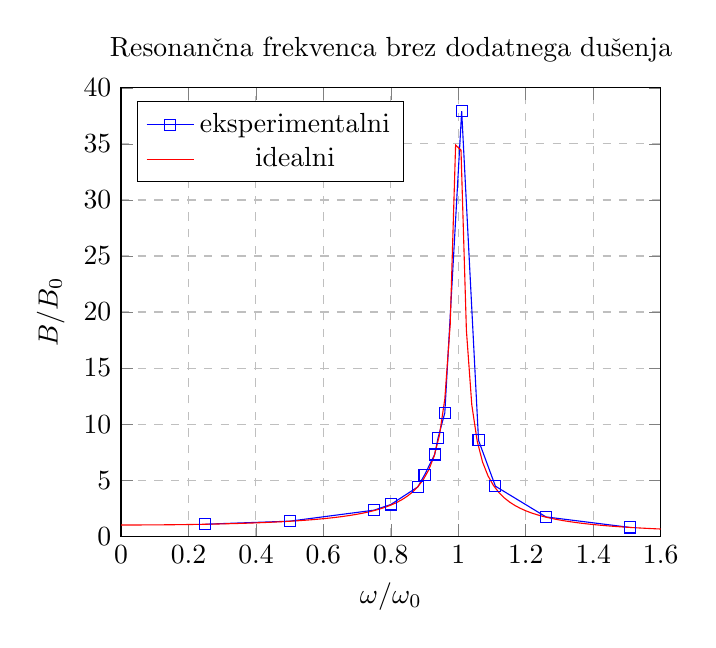
\begin{tikzpicture}
\begin{axis}[
    title={Resonančna frekvenca brez dodatnega dušenja},
    xlabel={$\omega/\omega_0$},
    ylabel={$B/B_0$},
    xmin=0, xmax=1.6,
    ymin=0, ymax=40,
    xtick={0,0.2,0.4,0.6,0.8,1,1.2,1.4,1.6},
    ytick={0,5,10,15,20,25,30,35,40},
    legend pos=north west,
    ymajorgrids=true,
    xmajorgrids=true,
    grid style=dashed,
]

\addplot[
    color=blue,
    mark=square,
    ]
    coordinates {
    (	0.25	,	1.07	)
(	0.50	,	1.34	)
(	0.75	,	2.32	)
(	0.80	,	2.83	)
(	0.88	,	4.40	)
(	0.90	,	5.47	)
(	0.93	,	7.29	)
(	0.94	,	8.77	)
(	0.96	,	11.01	)
(	1.01	,	37.92	)
(	1.06	,	8.55	)
(	1.11	,	4.46	)
(	1.26	,	1.72	)
(	1.51	,	0.78	)

    };
    \legend{eksperimentalni}

\addplot[
    color=red]
    %{1.000/((0.000576*x^2 + (1.000-x^2)^2)^(1/2))};
    %{1/sqrt((1-x*x)^2 + (2*0.03/2.5)^2 * x*x)};
    coordinates {
    (	0	,	1	)
(	0.016	,	1.000255992	)
(	0.032	,	1.001024754	)
(	0.048	,	1.002308653	)
(	0.064	,	1.004111652	)
(	0.08	,	1.006439345	)
(	0.096	,	1.009298996	)
(	0.112	,	1.012699599	)
(	0.128	,	1.016651948	)
(	0.144	,	1.021168727	)
(	0.16	,	1.026264609	)
(	0.176	,	1.03195638	)
(	0.192	,	1.038263085	)
(	0.208	,	1.045206188	)
(	0.224	,	1.052809765	)
(	0.24	,	1.061100724	)
(	0.256	,	1.070109053	)
(	0.272	,	1.079868115	)
(	0.288	,	1.090414977	)
(	0.304	,	1.101790787	)
(	0.32	,	1.114041219	)
(	0.336	,	1.127216974	)
(	0.352	,	1.14137436	)
(	0.368	,	1.156575971	)
(	0.384	,	1.17289146	)
(	0.4	,	1.190398453	)
(	0.416	,	1.209183602	)
(	0.432	,	1.229343832	)
(	0.448	,	1.25098779	)
(	0.464	,	1.27423757	)
(	0.48	,	1.299230751	)
(	0.496	,	1.326122823	)
(	0.512	,	1.355090094	)
(	0.528	,	1.386333189	)
(	0.544	,	1.420081283	)
(	0.56	,	1.456597259	)
(	0.576	,	1.496184032	)
(	0.592	,	1.539192359	)
(	0.608	,	1.586030556	)
(	0.624	,	1.637176691	)
(	0.64	,	1.693194019	)
(	0.656	,	1.754750708	)
(	0.672	,	1.822645319	)
(	0.688	,	1.897840092	)
(	0.704	,	1.981504973	)
(	0.72	,	2.07507666	)
(	0.736	,	2.180338988	)
(	0.752	,	2.299534221	)
(	0.768	,	2.435520041	)
(	0.784	,	2.59199569	)
(	0.8	,	2.773835569	)
(	0.816	,	2.987594803	)
(	0.832	,	3.242299661	)
(	0.848	,	3.550728769	)
(	0.864	,	3.931580082	)
(	0.88	,	4.413326781	)
(	0.896	,	5.041514376	)
(	0.912	,	5.893665147	)
(	0.928	,	7.112813822	)
(	0.944	,	8.99308764	)
(	0.96	,	12.23759994	)
(	0.976	,	18.90592414	)
(	0.992	,	34.90498226	)
(	1.008	,	34.43560144	)
(	1.024	,	18.36917508	)
(	1.04	,	11.71892395	)
(	1.056	,	8.482311338	)
(	1.072	,	6.605619853	)
(	1.088	,	5.388217752	)
(	1.104	,	4.53690996	)
(	1.12	,	3.909057589	)
(	1.136	,	3.427326591	)
(	1.152	,	3.046269411	)
(	1.168	,	2.737467583	)
(	1.184	,	2.482255461	)
(	1.2	,	2.267874341	)
(	1.216	,	2.085310645	)
(	1.232	,	1.928017518	)
(	1.248	,	1.791126018	)
(	1.264	,	1.6709405	)
(	1.28	,	1.564605616	)
(	1.296	,	1.469880539	)
(	1.312	,	1.384982224	)
(	1.328	,	1.308474277	)
(	1.344	,	1.239186682	)
(	1.36	,	1.176156829	)
(	1.376	,	1.118585544	)
(	1.392	,	1.06580384	)
(	1.408	,	1.017247463	)
(	1.424	,	0.972437182	)
(	1.44	,	0.930963375	)
(	1.456	,	0.892473837	)
(	1.472	,	0.856664073	)
(	1.488	,	0.823269488	)
(	1.504	,	0.792059069	)
(	1.52	,	0.762830224	)
(	1.536	,	0.735404546	)
(	1.552	,	0.709624315	)
(	1.568	,	0.685349586	)
(	1.584	,	0.662455757	)
(	1.6	,	0.640831525	)
};
    
\addlegendentry{idealni}
    
\end{axis}
\end{tikzpicture}
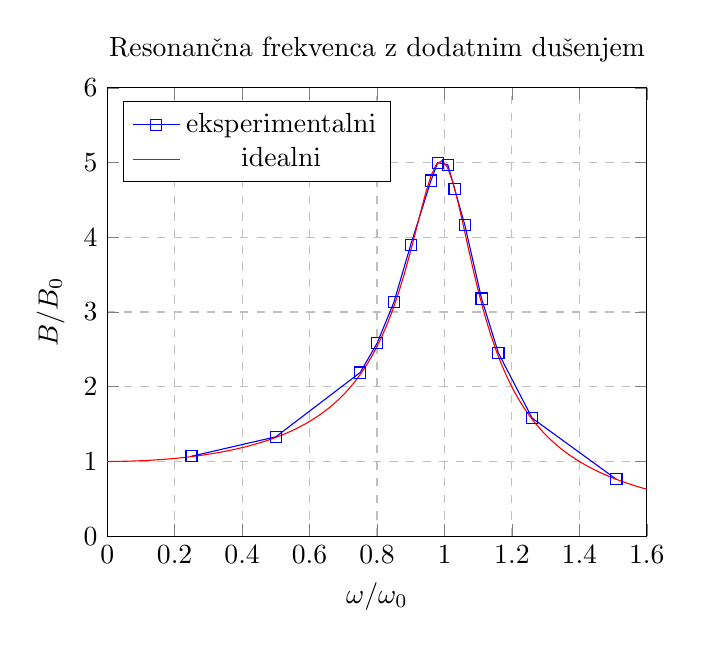
\begin{tikzpicture}
\begin{axis}[
    title={Resonančna frekvenca z dodatnim dušenjem},
    xlabel={$\omega/\omega_0$},
    ylabel={$B/B_0$},
    xmin=0, xmax=1.6,
    ymin=0, ymax=6,
    xtick={0,0.2,0.4,0.6,0.8,1,1.2,1.4,1.6},
    ytick={0,1,2,3,4,5,6},
    legend pos=north west,
    ymajorgrids=true,
    xmajorgrids=true,
    grid style=dashed,
]

\addplot[
    color=blue,
    mark=square,
    ]
    coordinates {
    	(	0.25	,	1.07	)
(	0.50	,	1.33	)
(	0.75	,	2.19	)
(	0.80	,	2.58	)
(	0.85	,	3.13	)
(	0.90	,	3.90	)
(	0.96	,	4.76	)
(	0.98	,	5.00	)
(	1.01	,	4.97	)
(	1.03	,	4.65	)
(	1.06	,	4.17	)
(	1.11	,	3.18	)
(	1.16	,	2.45	)
(	1.26	,	1.58	)
(	1.51	,	0.76	)


    };
    \legend{eksperimentalni}

\addplot[
    color=red]
    %{1.000/((0.000576*x^2 + (1.000-x^2)^2)^(1/2))};
    %{1/sqrt((1-x*x)^2 + (2*0.03/2.5)^2 * x*x)};
    coordinates {(	0	,	1	)
(	0.016	,	1.000250942	)
(	0.032	,	1.001004507	)
(	0.048	,	1.002262924	)
(	0.064	,	1.004029922	)
(	0.08	,	1.00631076	)
(	0.096	,	1.009112267	)
(	0.112	,	1.012442888	)
(	0.128	,	1.016312753	)
(	0.144	,	1.020733746	)
(	0.16	,	1.025719601	)
(	0.176	,	1.031286007	)
(	0.192	,	1.037450731	)
(	0.208	,	1.044233762	)
(	0.224	,	1.051657472	)
(	0.24	,	1.059746809	)
(	0.256	,	1.068529507	)
(	0.272	,	1.07803633	)
(	0.288	,	1.088301357	)
(	0.304	,	1.09936229	)
(	0.32	,	1.111260826	)
(	0.336	,	1.124043064	)
(	0.352	,	1.137759982	)
(	0.368	,	1.152467973	)
(	0.384	,	1.168229471	)
(	0.4	,	1.185113658	)
(	0.416	,	1.203197286	)
(	0.432	,	1.222565625	)
(	0.448	,	1.243313552	)
(	0.464	,	1.265546824	)
(	0.48	,	1.289383554	)
(	0.496	,	1.314955924	)
(	0.512	,	1.342412206	)
(	0.528	,	1.371919114	)
(	0.544	,	1.403664579	)
(	0.56	,	1.437861028	)
(	0.576	,	1.474749246	)
(	0.592	,	1.514602979	)
(	0.608	,	1.557734384	)
(	0.624	,	1.604500537	)
(	0.64	,	1.65531119	)
(	0.656	,	1.710638022	)
(	0.672	,	1.77102568	)
(	0.688	,	1.837104888	)
(	0.704	,	1.909607946	)
(	0.72	,	1.989386841	)
(	0.736	,	2.077434023	)
(	0.752	,	2.174905473	)
(	0.768	,	2.283144826	)
(	0.784	,	2.403705605	)
(	0.8	,	2.538365413	)
(	0.816	,	2.689119994	)
(	0.832	,	2.858134321	)
(	0.848	,	3.047609039	)
(	0.864	,	3.259489153	)
(	0.88	,	3.494893916	)
(	0.896	,	3.75308722	)
(	0.912	,	4.029774241	)
(	0.928	,	4.314625911	)
(	0.944	,	4.588468732	)
(	0.96	,	4.821836181	)
(	0.976	,	4.978139469	)
(	0.992	,	5.024141468	)
(	1.008	,	4.944644765	)
(	1.024	,	4.751000329	)
(	1.04	,	4.475603205	)
(	1.056	,	4.157231994	)
(	1.072	,	3.828546045	)
(	1.088	,	3.511223455	)
(	1.104	,	3.216896475	)
(	1.12	,	2.950181633	)
(	1.136	,	2.711553305	)
(	1.152	,	2.499365969	)
(	1.168	,	2.31107748	)
(	1.184	,	2.143917133	)
(	1.2	,	1.995217211	)
(	1.216	,	1.862556524	)
(	1.232	,	1.74380534	)
(	1.248	,	1.637122017	)
(	1.264	,	1.540928363	)
(	1.28	,	1.453877645	)
(	1.296	,	1.374822055	)
(	1.312	,	1.302782677	)
(	1.328	,	1.236923064	)
(	1.344	,	1.176526619	)
(	1.36	,	1.120977505	)
(	1.376	,	1.069744677	)
(	1.392	,	1.022368587	)
(	1.408	,	0.978450129	)
(	1.424	,	0.937641439	)
(	1.44	,	0.899638248	)
(	1.456	,	0.864173493	)
(	1.472	,	0.831011975	)
(	1.488	,	0.799945884	)
(	1.504	,	0.770791028	)
(	1.52	,	0.743383653	)
(	1.536	,	0.717577748	)
(	1.552	,	0.693242755	)
(	1.568	,	0.670261621	)
(	1.584	,	0.648529125	)
(	1.6	,	0.627950449	)
};
    
\addlegendentry{idealni}
    
\end{axis}
\end{tikzpicture}
\raggedright \normalsize


\subsection{Graf faznega zamika $\delta$($\omega/\omega_0$)}

Fazni zamik računamo s formulo:

\centering \large
\begin{equation}
     \tan(\delta) = \frac{a(\frac{\omega}{\omega_0})}{1-(\frac{\omega}{\omega_0})^2}
\end{equation}
\raggedright \normalsize

Tako bomo iz $\omega/\omega_0$ določili pravilni $\delta$, ter to primerjali z grafom funkcije, zgoraj omenjene enačbe, če je $\omega/\omega_0 = x$ 

\centering \large
\begin{tabular}{|p{1.5cm}|p{1.5cm}|p{1.5cm}|}
    \hline
    \multicolumn{3}{|c|}{1. Fazni zamik}\\
    \hline
    Index & $\delta_e$ & $\delta_i$ \\
    \hline
    1 & 0 & 0,06\\
    2 & 0 & 0,16\\
    3 & $\pi/16$ & 0,40\\
    4 & $\pi/8$ & 0,50\\
    5 & $\pi/4$ & 0,75\\
    6 & $\pi/2$ & 0,87 \\
    7 & $\pi/2$ & 1,03\\
    8 & $\pi/2$ & 1,11\\
    9 & $\pi/2$ & 1,20\\
    10 & $3\pi/4$ & 1,61\\
    11 & $\pi$ & 1,99\\
    12 & $\pi$ & 2,27\\
    13 & $\pi$ & 2,66\\
    14 & $\pi$ & 2,68\\
    \hline
\end{tabular}

\begin{tabular}{|p{1.5cm}|p{1.5cm}|p{1.5cm}|}
    \hline
    \multicolumn{3}{|c|}{2. Fazni zamik}\\
    \hline
    Index & $\delta_e$ & $\delta_i$ \\
    \hline
    1 & 0 & 0,05 \\
    2 & 0 & 0,13\\
    3 & 0 & 0,34\\
    4 & $\pi/4$ & 0,43\\
    5 & $\pi/4$ & 0,56\\
    6 & $\pi/2$ & 0,78\\
    7 & $\pi/2$ & 1,14\\
    8 & $\pi/2$ & 1,37\\
    9 & $\pi/2$ & 1,62\\
    10 & $\pi/2$ & 1,86\\
    11 & $\pi/2$ & 2,07\\
    12 & $3\pi/4$ & 2,36\\
    13 & $3\pi/4$ & 2,54\\
    14 & $\pi$ & 2,73\\
    15 & $\pi$ & 2,91\\
    \hline
\end{tabular}

\raggedright \normalsize

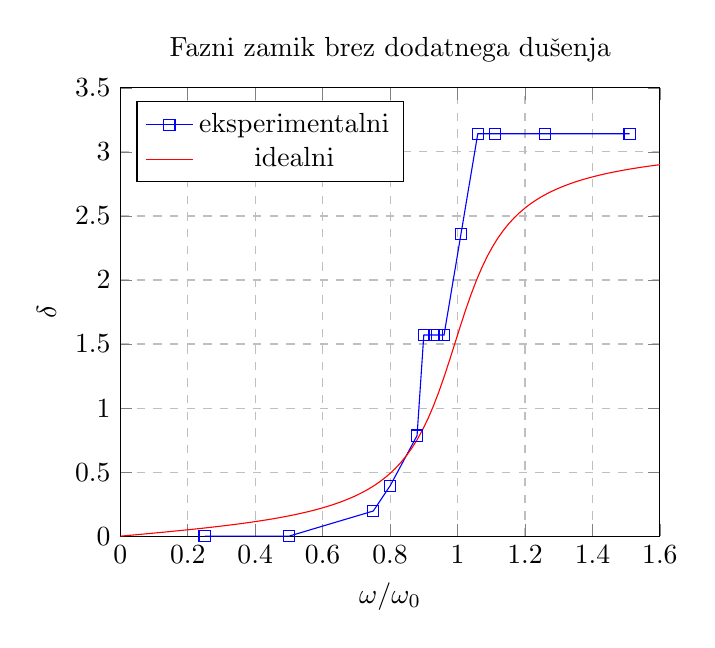
\begin{tikzpicture}
\begin{axis}[
    title={Fazni zamik brez dodatnega dušenja},
    xlabel={$\omega/\omega_0$},
    ylabel={$\delta$},
    xmin=0, xmax=1.6,
    ymin=0, ymax=3.5,
    xtick={0,0.2,0.4,0.6,0.8,1,1.2,1.4,1.6},
    ytick={0,0.5,1.0,1.5,2.0,2.5,3.0,3.5},
    legend pos=north west,
    ymajorgrids=true,
    xmajorgrids=true,
    grid style=dashed,
]

\addplot[
    color=blue,
    mark=square,
    ]
    coordinates { (	0.25	,	0	)
(	0.50	,	0	)
(	0.75	,	0.19634954084)
(	0.80	,	0.39269908169)
(	0.88	,	0.78539816339 	)
(	0.90	,	1.57079632679 	)
(	0.93	,	1.57079632679 	)
(	0.94	,	1.57079632679 	)
(	0.96	,	1.57079632679 	)
(	1.01	,	 2.35619449019 	)
(	1.06	,	3.14159265359 	)
(	1.11	,	3.14159265359 	)
(	1.26	,	3.14159265359 	)
(	1.51	,	3.14159265359 	)

    
    };
    \legend{eksperimentalni}

\addplot[
    color=red
    ]
    coordinates { (	0	,	0	)
(	0.016	,	0.003840964	)
(	0.032	,	0.007687721	)
(	0.048	,	0.01154609	)
(	0.064	,	0.015421951	)
(	0.08	,	0.019321267	)
(	0.096	,	0.023250121	)
(	0.112	,	0.027214745	)
(	0.128	,	0.031221551	)
(	0.144	,	0.03527717	)
(	0.16	,	0.039388485	)
(	0.176	,	0.043562674	)
(	0.192	,	0.047807256	)
(	0.208	,	0.05213013	)
(	0.224	,	0.056539635	)
(	0.24	,	0.061044604	)
(	0.256	,	0.065654424	)
(	0.272	,	0.07037911	)
(	0.288	,	0.075229383	)
(	0.304	,	0.080216752	)
(	0.32	,	0.085353618	)
(	0.336	,	0.090653382	)
(	0.352	,	0.096130573	)
(	0.368	,	0.101800986	)
(	0.384	,	0.107681849	)
(	0.4	,	0.113792007	)
(	0.416	,	0.120152137	)
(	0.432	,	0.126784994	)
(	0.448	,	0.133715694	)
(	0.464	,	0.140972049	)
(	0.48	,	0.148584946	)
(	0.496	,	0.1565888	)
(	0.512	,	0.165022084	)
(	0.528	,	0.173927944	)
(	0.544	,	0.183354936	)
(	0.56	,	0.193357897	)
(	0.576	,	0.203998977	)
(	0.592	,	0.215348884	)
(	0.608	,	0.227488365	)
(	0.624	,	0.240509998	)
(	0.64	,	0.254520358	)
(	0.656	,	0.269642639	)
(	0.672	,	0.286019851	)
(	0.688	,	0.303818711	)
(	0.704	,	0.323234402	)
(	0.72	,	0.344496384	)
(	0.736	,	0.36787547	)
(	0.752	,	0.393692426	)
(	0.768	,	0.422328293	)
(	0.784	,	0.454236593	)
(	0.8	,	0.489957326	)
(	0.816	,	0.530132206	)
(	0.832	,	0.575519582	)
(	0.848	,	0.627005705	)
(	0.864	,	0.685605767	)
(	0.88	,	0.752443066	)
(	0.896	,	0.828687358	)
(	0.912	,	0.915425789	)
(	0.928	,	1.013437802	)
(	0.944	,	1.122863174	)
(	0.96	,	1.242808847	)
(	0.976	,	1.37103745	)
(	0.992	,	1.50396054	)
(	1.008	,	1.637101106	)
(	1.024	,	1.765937268	)
(	1.04	,	1.886766599	)
(	1.056	,	1.997214515	)
(	1.072	,	2.09626843	)
(	1.088	,	2.183985462	)
(	1.104	,	2.261099196	)
(	1.12	,	2.328678501	)
(	1.136	,	2.387892019	)
(	1.152	,	2.439870983	)
(	1.168	,	2.485642322	)
(	1.184	,	2.52610482	)
(	1.2	,	2.562028668	)
(	1.216	,	2.594066078	)
(	1.232	,	2.622766041	)
(	1.248	,	2.648589621	)
(	1.264	,	2.671924108	)
(	1.28	,	2.6930954	)
(	1.296	,	2.712378513	)
(	1.312	,	2.730006326	)
(	1.328	,	2.746176802	)
(	1.344	,	2.761058907	)
(	1.36	,	2.774797464	)
(	1.376	,	2.787517117	)
(	1.392	,	2.799325588	)
(	1.408	,	2.810316351	)
(	1.424	,	2.820570839	)
(	1.44	,	2.830160261	)
(	1.456	,	2.839147118	)
(	1.472	,	2.847586461	)
(	1.488	,	2.855526943	)
(	1.504	,	2.863011706	)
(	1.52	,	2.870079124	)
(	1.536	,	2.87676343	)
(	1.552	,	2.883095254	)
(	1.568	,	2.889102075	)
(	1.584	,	2.894808614	)
(	1.6	,	2.900237163	)

    
    };
    
\addlegendentry{idealni}
    
\end{axis}
\end{tikzpicture}

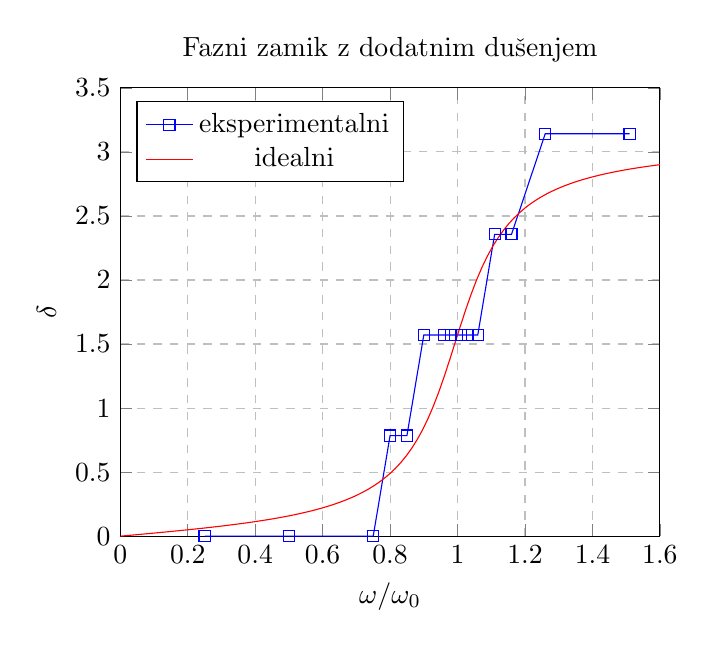
\begin{tikzpicture}
\begin{axis}[
    title={Fazni zamik z dodatnim dušenjem},
    xlabel={$\omega/\omega_0$},
    ylabel={$\delta$},
    xmin=0, xmax=1.6,
    ymin=0, ymax=3.5,
    xtick={0,0.2,0.4,0.6,0.8,1,1.2,1.4,1.6},
    ytick={0,0.5,1.0,1.5,2.0,2.5,3.0,3.5},
    legend pos=north west,
    ymajorgrids=true,
    xmajorgrids=true,
    grid style=dashed,
]

\addplot[
    color=blue,
    mark=square,
    ]
    coordinates { (	0.25	,	0	)
(	0.50	,	0	)
(	0.75	,	0	)
(	0.80	,	0.78539816339	)
(	0.85	,	0.78539816339	)
(	0.90	,	1.57079632679	)
(	0.96	,	1.57079632679	)
(	0.98	,	1.57079632679	)
(	1.01	,	1.57079632679	)
(	1.03	,	1.57079632679	)
(	1.06	,	1.57079632679	)
(	1.11	,	2.35619449019	)
(	1.16	,	2.35619449019	)
(	1.26	,	3.14159265359	)
(	1.51	,	3.14159265359	)

    };
    \legend{eksperimentalni}

\addplot[
    color=red
    ]
    coordinates { (	0	,	0	)
(	0.016	,	0.003840964	)
(	0.032	,	0.007687721	)
(	0.048	,	0.01154609	)
(	0.064	,	0.015421951	)
(	0.08	,	0.019321267	)
(	0.096	,	0.023250121	)
(	0.112	,	0.027214745	)
(	0.128	,	0.031221551	)
(	0.144	,	0.03527717	)
(	0.16	,	0.039388485	)
(	0.176	,	0.043562674	)
(	0.192	,	0.047807256	)
(	0.208	,	0.05213013	)
(	0.224	,	0.056539635	)
(	0.24	,	0.061044604	)
(	0.256	,	0.065654424	)
(	0.272	,	0.07037911	)
(	0.288	,	0.075229383	)
(	0.304	,	0.080216752	)
(	0.32	,	0.085353618	)
(	0.336	,	0.090653382	)
(	0.352	,	0.096130573	)
(	0.368	,	0.101800986	)
(	0.384	,	0.107681849	)
(	0.4	,	0.113792007	)
(	0.416	,	0.120152137	)
(	0.432	,	0.126784994	)
(	0.448	,	0.133715694	)
(	0.464	,	0.140972049	)
(	0.48	,	0.148584946	)
(	0.496	,	0.1565888	)
(	0.512	,	0.165022084	)
(	0.528	,	0.173927944	)
(	0.544	,	0.183354936	)
(	0.56	,	0.193357897	)
(	0.576	,	0.203998977	)
(	0.592	,	0.215348884	)
(	0.608	,	0.227488365	)
(	0.624	,	0.240509998	)
(	0.64	,	0.254520358	)
(	0.656	,	0.269642639	)
(	0.672	,	0.286019851	)
(	0.688	,	0.303818711	)
(	0.704	,	0.323234402	)
(	0.72	,	0.344496384	)
(	0.736	,	0.36787547	)
(	0.752	,	0.393692426	)
(	0.768	,	0.422328293	)
(	0.784	,	0.454236593	)
(	0.8	,	0.489957326	)
(	0.816	,	0.530132206	)
(	0.832	,	0.575519582	)
(	0.848	,	0.627005705	)
(	0.864	,	0.685605767	)
(	0.88	,	0.752443066	)
(	0.896	,	0.828687358	)
(	0.912	,	0.915425789	)
(	0.928	,	1.013437802	)
(	0.944	,	1.122863174	)
(	0.96	,	1.242808847	)
(	0.976	,	1.37103745	)
(	0.992	,	1.50396054	)
(	1.008	,	1.637101106	)
(	1.024	,	1.765937268	)
(	1.04	,	1.886766599	)
(	1.056	,	1.997214515	)
(	1.072	,	2.09626843	)
(	1.088	,	2.183985462	)
(	1.104	,	2.261099196	)
(	1.12	,	2.328678501	)
(	1.136	,	2.387892019	)
(	1.152	,	2.439870983	)
(	1.168	,	2.485642322	)
(	1.184	,	2.52610482	)
(	1.2	,	2.562028668	)
(	1.216	,	2.594066078	)
(	1.232	,	2.622766041	)
(	1.248	,	2.648589621	)
(	1.264	,	2.671924108	)
(	1.28	,	2.6930954	)
(	1.296	,	2.712378513	)
(	1.312	,	2.730006326	)
(	1.328	,	2.746176802	)
(	1.344	,	2.761058907	)
(	1.36	,	2.774797464	)
(	1.376	,	2.787517117	)
(	1.392	,	2.799325588	)
(	1.408	,	2.810316351	)
(	1.424	,	2.820570839	)
(	1.44	,	2.830160261	)
(	1.456	,	2.839147118	)
(	1.472	,	2.847586461	)
(	1.488	,	2.855526943	)
(	1.504	,	2.863011706	)
(	1.52	,	2.870079124	)
(	1.536	,	2.87676343	)
(	1.552	,	2.883095254	)
(	1.568	,	2.889102075	)
(	1.584	,	2.894808614	)
(	1.6	,	2.900237163	)

    
    };
    
\addlegendentry{idealni}
    
\end{axis}
\end{tikzpicture}

\subsection{Povprečna sprejeta moč - $\frac{\overline{P}}{M_0 B_0 \omega_0}$($\omega/\omega_0$)}

Povrpečno sprejeto moč izračunamo s formulo:

\centering \Large
\begin{equation}
    \overline{P} = \frac{1}{2}\omega M_0 B \sin{(\delta)}
\end{equation}
\raggedright \normalsize

iz česar sledi

\centering \Large
\begin{equation}
    \frac{\overline{P}}{M_0B_0\omega_O} = \frac{1}{2} \frac{\omega}{\omega_0} \frac{B}{B_0} \sin(\delta)
\end{equation}
\raggedright \normalsize

Za podatke lahko izračunamo:

\centering \large
\begin{tabular}{|p{1.5cm}|p{1.5cm}|p{1.5cm}|p{1.5cm}|p{1.5cm}|}
    \hline
    \multicolumn{5}{|c|}{1. Povprečna sprejeta moč}\\
    \hline
    Index & $\frac{\omega}{\omega_0}$ & $\frac{B}{B_0}$ & $\delta$ izr. & $\frac{\overline{P}}{M_0 B_0 \omega_0}$\\ 
    \hline
    1 & 0,25 & 1,07 & 0,06 & 0,01\\
    2 & 0,50 & 1,34 & 0,16 & 0,05\\
    3 & 0,75 & 2,32 & 0,40 & 0,34\\
    4 & 0,80 & 2,83 & 0,50 & 0,55\\
    5 & 0,86 & 4,40 & 0,75 & 1,32\\
    6 & 0,91 & 5,47 & 0,87 & 1,90\\
    7 & 0,93 & 7,29 & 1,03 & 2,90\\
    8 & 0,94 & 8,77 & 1,11 & 3,71\\
    9 & 0,96 & 11,01 & 1,20 & 4,91\\
    10 & 1,01 & 37,92 & 1,61 & 19,04\\
    11 & 1,06 & 8,55 & 1,99 & 4,11\\
    12 & 1,11 & 4,46 & 2,27 & 1,89\\
    13 & 1,26 & 1,72 & 2,66 & 0,50\\
    14 & 1,51 & 0,78 & 2,68 & 0,16\\
    \hline
\end{tabular}

\begin{tabular}{|p{1.5cm}|p{1.5cm}|p{1.5cm}|p{1.5cm}|p{1.5cm}|}
    \hline
    \multicolumn{5}{|c|}{2. Povprečna sprejeta moč}\\
    \hline
    Index & $\frac{\omega}{\omega_0}$ & $\frac{B}{B_0}$ & $\delta$ izr. & $\frac{\overline{P}}{M_0 B_0 \omega_0}$\\
    \hline
    1 & 0,25 & 1,07 & 0,05 & 0,01\\
    2 & 0,50 & 1,33 & 0,13 & 0,04\\
    3 & 0,75 & 2,19 & 0,34 & 0,27\\
    4 & 0,80 & 2,58 & 0,43 & 0,43\\
    5 & 0,86 & 3,13 & 0,56 & 0,72\\
    6 & 0,91 & 3,90 & 0,78 & 1,25\\
    7 & 0,96 & 4,76 & 1,14 & 2,06\\
    8 & 0,98 & 5,00 & 1,37 & 2,40\\
    9 & 1,01 & 4,97 & 1,62 & 2,49 \\
    10 & 1,03 & 4,65 & 1,86 & 2,29\\
    11 & 1,06 & 4,17 & 2,07 & 1,93\\
    12 & 1,11 & 3,18 & 2,36 & 1,24\\
    13 & 1,16 & 2,45 & 2,54 & 0,80\\
    14 & 1,26 & 1,58 & 2,73 & 0,40\\
    15 & 1,51 & 0,76 & 2,91 & 0,13 \\
    \hline
\end{tabular}
\large\centering
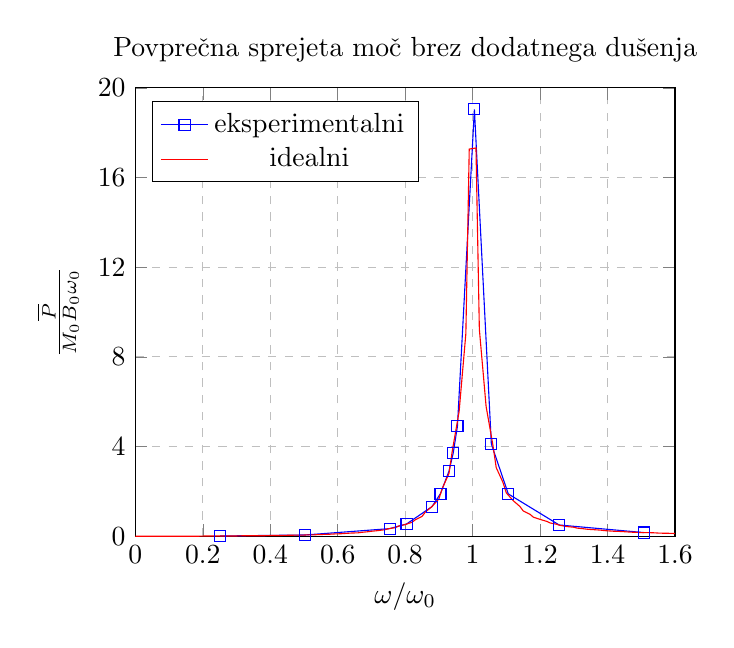
\begin{tikzpicture}
\begin{axis}[
    title={Povprečna sprejeta moč brez dodatnega dušenja},
    xlabel={$\omega/\omega_0$},
    ylabel={$\frac{\overline{P}}{M_0 B_0 \omega_0}$},
    xmin=0, xmax=1.6,
    ymin=0, ymax=20,
    xtick={0,0.2,0.4,0.6,0.8,1,1.2,1.4,1.6},
    ytick={0,4,8,12,16,20},
    legend pos=north west,
    ymajorgrids=true,
    xmajorgrids=true,
    grid style=dashed,
]

\addplot[
    color=blue,
    mark=square,
    ]
    coordinates { (	0.251327412	,	0.008618424	)
(	0.502654825	,	0.053585133	)
(	0.753982237	,	0.337567979	)
(	0.804247719	,	0.545201959	)
(	0.879645943	,	1.320736235	)
(	0.904778684	,	1.900713369	)
(	0.929911425	,	2.900393859	)
(	0.942477796	,	3.70608328	)
(	0.955044167	,	4.908793818	)
(	1.005309649	,	19.04136956	)
(	1.055575132	,	4.111744655	)
(	1.105840614	,	1.886393404	)
(	1.256637061	,	0.500431672	)
(	1.507964474	,	0.16166852	)

    
    };
    \legend{eksperimentalni}

\addplot[
    color=red
    ]
    coordinates { 
(	0.00	,	0.00	)
(	0.02	,	0.00	)
(	0.03	,	0.00	)
(	0.05	,	0.00	)
(	0.06	,	0.00	)
(	0.08	,	0.00	)
(	0.10	,	0.00	)
(	0.11	,	0.00	)
(	0.13	,	0.00	)
(	0.14	,	0.00	)
(	0.16	,	0.00	)
(	0.18	,	0.00	)
(	0.19	,	0.00	)
(	0.21	,	0.01	)
(	0.22	,	0.01	)
(	0.24	,	0.01	)
(	0.26	,	0.01	)
(	0.27	,	0.01	)
(	0.29	,	0.01	)
(	0.30	,	0.01	)
(	0.32	,	0.02	)
(	0.34	,	0.02	)
(	0.35	,	0.02	)
(	0.37	,	0.02	)
(	0.38	,	0.02	)
(	0.40	,	0.03	)
(	0.42	,	0.03	)
(	0.43	,	0.03	)
(	0.45	,	0.04	)
(	0.46	,	0.04	)
(	0.48	,	0.05	)
(	0.50	,	0.05	)
(	0.51	,	0.06	)
(	0.53	,	0.06	)
(	0.54	,	0.07	)
(	0.56	,	0.08	)
(	0.58	,	0.09	)
(	0.59	,	0.10	)
(	0.61	,	0.11	)
(	0.62	,	0.12	)
(	0.64	,	0.14	)
(	0.66	,	0.15	)
(	0.67	,	0.17	)
(	0.69	,	0.20	)
(	0.70	,	0.22	)
(	0.72	,	0.25	)
(	0.74	,	0.29	)
(	0.75	,	0.33	)
(	0.77	,	0.38	)
(	0.78	,	0.45	)
(	0.80	,	0.52	)
(	0.82	,	0.62	)
(	0.83	,	0.73	)
(	0.85	,	0.88	)
(	0.86	,	1.08	)
(	0.88	,	1.33	)
(	0.90	,	1.66	)
(	0.91	,	2.13	)
(	0.93	,	2.80	)
(	0.94	,	3.83	)
(	0.96	,	5.56	)
(	0.98	,	9.04	)
(	0.99	,	17.27	)
(	1.01	,	17.32	)
(	1.02	,	9.23	)
(	1.04	,	5.79	)
(	1.06	,	4.08	)
(	1.07	,	3.06	)
(	1.09	,	2.40	)
(	1.10	,	1.93	)
(	1.12	,	1.59	)
(	1.14	,	1.33	)
(	1.15	,	1.13	)
(	1.17	,	0.98	)
(	1.18	,	0.85	)
(	1.20	,	0.75	)
(	1.22	,	0.66	)
(	1.23	,	0.59	)
(	1.25	,	0.53	)
(	1.26	,	0.48	)
(	1.28	,	0.43	)
(	1.30	,	0.40	)
(	1.31	,	0.36	)
(	1.33	,	0.33	)
(	1.34	,	0.31	)
(	1.36	,	0.29	)
(	1.38	,	0.27	)
(	1.39	,	0.25	)
(	1.41	,	0.23	)
(	1.42	,	0.22	)
(	1.44	,	0.21	)
(	1.46	,	0.19	)
(	1.47	,	0.18	)
(	1.49	,	0.17	)
(	1.50	,	0.16	)
(	1.52	,	0.16	)
(	1.54	,	0.15	)
(	1.55	,	0.14	)
(	1.57	,	0.13	)
(	1.58	,	0.13	)
(	1.60	,	0.12	)

    
    };
    
\addlegendentry{idealni}
    
\end{axis}
\end{tikzpicture}

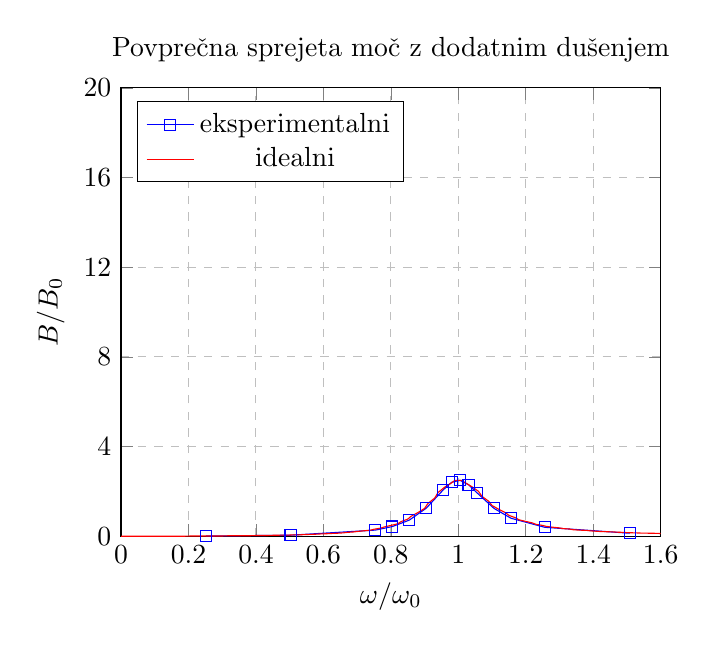
\begin{tikzpicture}
\begin{axis}[
    title={Povprečna sprejeta moč z dodatnim dušenjem},
    xlabel={$\omega/\omega_0$},
    ylabel={$B/B_0$},
    xmin=0, xmax=1.6,
    ymin=0, ymax=20,
    xtick={0,0.2,0.4,0.6,0.8,1,1.2,1.4,1.6},
    ytick={0,4,8,12,16,20},
    legend pos=north west,
    ymajorgrids=true,
    xmajorgrids=true,
    grid style=dashed,
]

\addplot[
    color=blue,
    mark=square,
    ]
    coordinates { (	0.251327412	,	0.007176381	)
(	0.502654825	,	0.044434163	)
(	0.753982237	,	0.27208105	)
(	0.804247719	,	0.429455562	)
(	0.854513202	,	0.715849822	)
(	0.904778684	,	1.247103513	)
(	0.955044167	,	2.063169249	)
(	0.980176908	,	2.403628376	)
(	1.005309649	,	2.493008689	)
(	1.03044239	,	2.29367001	)
(	1.055575132	,	1.933768627	)
(	1.105840614	,	1.240342815	)
(	1.156106097	,	0.801546913	)
(	1.256637061	,	0.396205772	)
(	1.507964474	,	0.132675451	)

    };
    \legend{eksperimentalni}

\addplot[
    color=red
    ]
    coordinates { (	0.00	,	0.00	)
(	0.02	,	0.00	)
(	0.03	,	0.00	)
(	0.05	,	0.00	)
(	0.06	,	0.00	)
(	0.08	,	0.00	)
(	0.10	,	0.00	)
(	0.11	,	0.00	)
(	0.13	,	0.00	)
(	0.14	,	0.00	)
(	0.16	,	0.00	)
(	0.18	,	0.00	)
(	0.19	,	0.00	)
(	0.21	,	0.01	)
(	0.22	,	0.01	)
(	0.24	,	0.01	)
(	0.26	,	0.01	)
(	0.27	,	0.01	)
(	0.29	,	0.01	)
(	0.30	,	0.01	)
(	0.32	,	0.02	)
(	0.34	,	0.02	)
(	0.35	,	0.02	)
(	0.37	,	0.02	)
(	0.38	,	0.02	)
(	0.40	,	0.03	)
(	0.42	,	0.03	)
(	0.43	,	0.03	)
(	0.45	,	0.04	)
(	0.46	,	0.04	)
(	0.48	,	0.05	)
(	0.50	,	0.05	)
(	0.51	,	0.06	)
(	0.53	,	0.06	)
(	0.54	,	0.07	)
(	0.56	,	0.08	)
(	0.58	,	0.09	)
(	0.59	,	0.10	)
(	0.61	,	0.11	)
(	0.62	,	0.12	)
(	0.64	,	0.13	)
(	0.66	,	0.15	)
(	0.67	,	0.17	)
(	0.69	,	0.19	)
(	0.70	,	0.21	)
(	0.72	,	0.24	)
(	0.74	,	0.27	)
(	0.75	,	0.31	)
(	0.77	,	0.36	)
(	0.78	,	0.41	)
(	0.80	,	0.48	)
(	0.82	,	0.55	)
(	0.83	,	0.65	)
(	0.85	,	0.76	)
(	0.86	,	0.89	)
(	0.88	,	1.05	)
(	0.90	,	1.24	)
(	0.91	,	1.46	)
(	0.93	,	1.70	)
(	0.94	,	1.95	)
(	0.96	,	2.19	)
(	0.98	,	2.38	)
(	0.99	,	2.49	)
(	1.01	,	2.49	)
(	1.02	,	2.39	)
(	1.04	,	2.21	)
(	1.06	,	2.00	)
(	1.07	,	1.78	)
(	1.09	,	1.56	)
(	1.10	,	1.37	)
(	1.12	,	1.20	)
(	1.14	,	1.05	)
(	1.15	,	0.93	)
(	1.17	,	0.82	)
(	1.18	,	0.73	)
(	1.20	,	0.66	)
(	1.22	,	0.59	)
(	1.23	,	0.53	)
(	1.25	,	0.48	)
(	1.26	,	0.44	)
(	1.28	,	0.40	)
(	1.30	,	0.37	)
(	1.31	,	0.34	)
(	1.33	,	0.32	)
(	1.34	,	0.29	)
(	1.36	,	0.27	)
(	1.38	,	0.26	)
(	1.39	,	0.24	)
(	1.41	,	0.22	)
(	1.42	,	0.21	)
(	1.44	,	0.20	)
(	1.46	,	0.19	)
(	1.47	,	0.18	)
(	1.49	,	0.17	)
(	1.50	,	0.16	)
(	1.52	,	0.15	)
(	1.54	,	0.14	)
(	1.55	,	0.14	)
(	1.57	,	0.13	)
(	1.58	,	0.13	)
(	1.60	,	0.12	)
    
    };
    
\addlegendentry{idealni}
    
\end{axis}
\end{tikzpicture}

\raggedright
\normalsize
